% coding:utf-8

%FOSAET, a LaTeX-Code for a electrical summary of basic electronics
%Copyright (C) 2013, Daniel Winz, Ervin Mazlagic, Mario Felder

%This program is free software; you can redistribute it and/or
%modify it under the terms of the GNU General Public License
%as published by the Free Software Foundation; either version 2
%of the License, or (at your option) any later version.

%This program is distributed in the hope that it will be useful,
%but WITHOUT ANY WARRANTY; without even the implied warranty of
%MERCHANTABILITY or FITNESS FOR A PARTICULAR PURPOSE.  See the
%GNU General Public License for more details.
%----------------------------------------

\subsection{Source Schaltung mit Stromgegenkopplung}
\begin{figure}[h!]
	\centering
	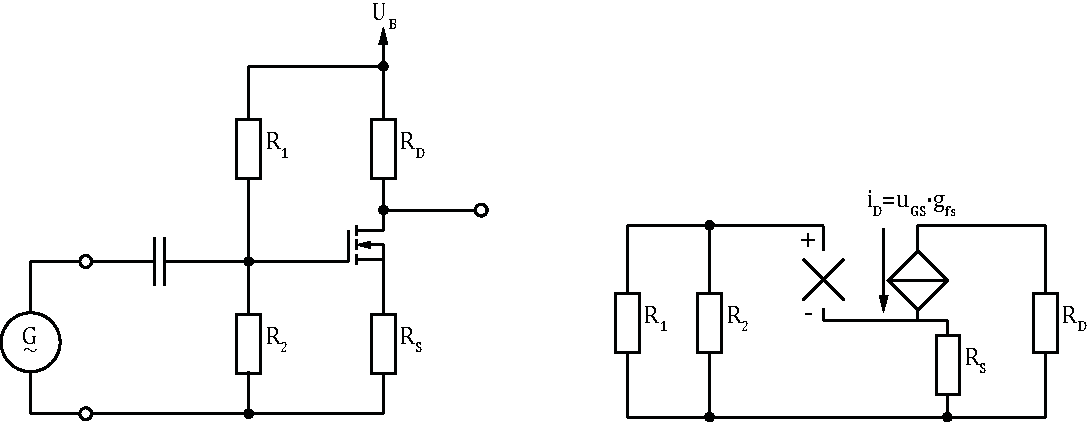
\includegraphics[width = \linewidth]{fet_source_i.pdf}
	\caption{Source Schaltung mit Stromgegenkopplung und Kleinsignalersatzschaltung}
	\label{fet:sourceschaltung_i}
\end{figure}
\noindent
\paragraph{Dimensionierung:}
\begin{itemize}
	\item Wahl von $I_D$ aufgrund des nötigen Ausgangswiderstandes $\rightarrow R_D$
	\item Wahl von $R_S$ für ein $U_{RS}$ von ca. $1V$
	\item Wahl von $R_2$ im Bereich von $100k\Omega$ bis $10M\Omega$
	\item $R_1 = R_2 \cdot \frac{U_B - U_{GS} - U_{RS}}{(U_{GS}+U_{RS})}$
	\item Untere Grenfrequenz: $f_{gu} = \frac{1}{2\pi \cdot C_2 \cdot R_1 \parallel R_2}$
\end{itemize}
\noindent\\
Spannungsverstärkung:
\[
	V_u = \frac{U_a}{U_e} = \frac{-g_{fs} \cdot R_D}{R_S \cdot g_{fs} + 1}
\]
Eingangswiderstand:
\[
	r_e = R_1 \parallel R_2
\]
Ausgangswiderstand:
\[
	r_a = R_D
\]
(Annahme: $r_{DS} \gg R_D$)